\documentclass[10pt,a4paper]{report}
\addtolength{\textheight}{-2cm}
\addtolength{\textwidth}{+2cm}
%------------------------------------------------------------------------------------------------------
\usepackage{xltxtra,fontspec,xunicode}
\usepackage[slantfont,boldfont]{xeCJK} % 允许斜体和粗体

\setCJKmainfont{WenQuanYi Micro Hei}             % 缺省中文字体
\setCJKmonofont{WenQuanYi Micro Hei Mono}        % 中文等宽字体
\setmainfont{DejaVu Serif}                       % 英文衬线字体
\setsansfont{DejaVu Sans}                        % 英文无衬线字体
\setmonofont{Monaco}                             % 英文等宽字体
%-------------------------------------------------------------------------------------------------------
\linespread{1.3}                                 % 1.5倍行距,值1.6产生双倍行距
% \setlength{\parindent}{0pt}                    % 段落首行缩进
\setlength{\parskip}{1ex plus 0.5ex minus 0.2ex} % 段落间距为1ex,可让TeX在+0.5到-0.8范围内微调
                                                 % 即实际范围在0.8ex~1.5ex之间
%-------------------------------------------------------------------------------------------------------
% 页眉与页脚设置
\usepackage{fancyhdr}
\pagestyle{fancy}
\fancyhf{}                                       %清空页眉页脚
\fancyhead[LE,RO]{\thepage}                      %页眉偶数页左,奇数页右
\fancyhead[RE]{\leftmark}                        %页眉偶数页右
\fancyhead[LO]{\rightmark}                       %页眉奇数页左
% \fancyfoot[LE,RO]{\thepage}                    %页脚偶数页左,奇数页右
% \fancyfoot[RE]{\leftmark}                      %页脚偶数页右
% \fancyfoot[LO]{\rightmark}                     %页脚奇数页左
\fancypagestyle{plain}{                          %重定义plain页面样式
    \fancyhf{}
    \renewcommand{\headrulewidth}{0pt}
}
%-------------------------------------------------------------------------------------------------------
% listings 与 xcolor 配合实现源代码的语法高亮
\usepackage{xcolor}
\usepackage{listings}
\lstset{
	language=Python,
	frame = shadowbox,
	basicstyle = \ttfamily\small,
	columns = fixed,
	numbers = left,
	numberstyle = \footnotesize,
	stepnumber = 1,
	tabsize = 2,
	showspaces = false,
	showstringspaces = false,
	showtabs = false,
	captionpos = b,
	breaklines = tr[],
	breakatwhitespace = false,
	backgroundcolor = \color{white},
	keywordstyle=\color{blue},
	numberstyle=\color[RGB]{0,192,192},
	commentstyle=\color[RGB]{0,96,96},
	stringstyle=\ttfamily\slshape\color[RGB]{128,0,0},
	escapeinside=``
}
%-------------------------------------------------------------------------------------------------------
\usepackage{graphicx}                            % 引入图片
\graphicspath{{img/}{images/}}                   % 要导入的图片的位置。可以有多个目录,但就算只有一个目录,也要用两级花括号
%-------------------------------------------------------------------------------------------------------
	\title{VIM学习笔记}                             % 文章的标题
	\author{                                     % 作者与致谢
		阿左 \thanks{感谢读者} \and 
		Nobody \thanks{感谢国家}
	}
	\date{\today}                                % 日期
	
%-------------------------------------------------------------------------------------------------------
\begin{document}
	\maketitle                                   % 制作标题
	\tableofcontents                             % 生成章节目录
	\setcounter{tocdepth}{5}                     % 生成章节的目录深度
	\listoffigures                               % 生成图片目录
	\listoftables                                % 生成表格目录


	\begin{abstract}                             % 英文摘要
		part of vim tech
	\end{abstract}

	\renewcommand{\abstractname}{摘要}           % 中文摘要
	\begin{abstract}

		部分vim技巧

	\end{abstract}

	\part{调用python脚本}
		
\chapter{调用python脚本}

	\section{基本介绍}

		先把函数定义于\verb|~/.vimrc|配置文件中。可以直接\verb|:so %|来重新载入,但是前提是所有在vimrc中的自定义函数都要定义成\verb|function!|这种形式。 

		\subsection{在状态栏显示信息}

			一个简单的例子:定义一个在vim的状态行中显示"Eat Me"的消息的函数。然后绑定到\verb|F7|键上。

			\lstinputlisting[language=python]{script/callpy/ShowEatMe.vim}

		\subsection{取得打开文件的缓存}

			下面函数从打开文件的缓存中取得文件内容,然后统计空白行的行数。

			\lstinputlisting[language=python]{script/callpy/CountBlankLine.vim}

		\subsection{调用python脚本}

			对于一个已经存在的python脚本:

			\lstinputlisting[language=python]{script/callpy/ShowEatMe.py}

			可以通过\verb|:pyfile <文件名>|来调用已经存在的python脚本。

			同样对于python脚本:

			\lstinputlisting[language=python]{script/callpy/CountBlankLine.py}

			也可以通过\verb|pyfile|命令调用。

	\section{vim模块}

		现在有了vim模块提供python程序对vim的操作。

		\subsection{基本常量}

			基本常量

			\lstinputlisting[language=python]{script/callpy/vimobj.txt}

			Python脚本的全部\verb|sys.stdout|输出都在vim的消息区,正常输出像是提示信息。所以的\verb|sts.stderr|错误信息像是错误提示。

			vim调用的python脚本不支持输入\verb|sys.stdin|(包括\verb|inout()|、\verb|raw_input()|),调用时很可能会发生错误。

		\subsection{错误对象}

			vim模块中的错误会抛出\verb|vim.err|类型的异常:

			\lstinputlisting[language=python]{script/callpy/vimerr.txt}

		\subsection{缓冲区对象}

			缓冲区对象可以通过以下途径获得:

			- via vim.current.buffer (|python-current|)

			- from indexing vim.buffers (|python-buffers|)

			- from the "buffer" attribute of a window (|python-window|)

			缓冲区对象可以作为一个序列对象。注意在索引与分片操作时结果会有不同:
			
			\verb|b[:]|的结果为\verb|None|,会清空整个缓冲区;\verb|b = None|仅仅更新了变量,不会影响缓冲区。

			缓存对象的常用的操作:
			\begin{verbatim}
				b.append(str)      Append a line to the buffer
				b.append(str, nr)  Idem, below line "nr"
				b.append(list)     Append a list of lines to the buffer
				                   Note that the option of supplying a list of strings to
				                   the append method differs from the equivalent method
				                   for Python's built-in list objects.
				b.append(list, nr) Idem, below line "nr"
				b.mark(name)       Return a tuple (row,col) representing the position
				                   of the named mark (can also get the []"<> marks)
				b.range(s,e)       Return a range object (see |python-range|) which
				                   represents the part of the given buffer between line
				                   numbers s and e |inclusive|.
			\end{verbatim}

			注意:用\verb|append()|添加一个新行时,不可以加上换行符\verb|'\n'|。 行尾可以有\verb|'\n'|但是会被忽略。所以以下的操作是被允许的:
			\begin{verbatim}
				:py b.append(f.readlines())
			\end{verbatim}

			常用的例子:

			\begin{verbatim}
				:py print b.name            # write the buffer file name
				:py b[0] = "hello!!!"       # replace the top line
				:py b[:] = None             # delete the whole buffer
				:py del b[:]                # delete the whole buffer
				:py b[0:0] = [ "a line" ]   # add a line at the top
				:py del b[2]                # delete a line (the third)
				:py b.append("bottom")      # add a line at the bottom
				:py n = len(b)              # number of lines
				:py (row,col) = b.mark('a') # named mark
				:py r = b.range(1,5)        # a sub-range of the buffer
			\end{verbatim}

		\subsection{范围对象}

			范围对象代表了一部分的缓冲区,取得方法有:

				- via vim.current.range (|python-current|)
				- from a buffer's range() method (|python-buffer|)

			常用属性有:
			\begin{verbatim}
				r.start     Index of first line into the buffer
				r.end       Index of last line into the buffer
			\end{verbatim}

			常用方法有:
			\begin{verbatim}
				r.append(str)      Append a line to the range
				r.append(str, nr)  Idem, after line "nr"
				r.append(list)     Append a list of lines to the range
				                   Note that the option of supplying a list of strings to
				                   the append method differs from the equivalent method
				                   for Python's built-in list objects.
				r.append(list, nr) Idem, after line "nr"
			\end{verbatim}

			例子(r是当前的范围):
			\begin{verbatim}
				# Send all lines in a range to the default printer
				vim.command("%d,%dhardcopy!" % (r.start+1,r.end+1))
			\end{verbatim}

		\subsection{窗口对象}

			窗口对象代表了一个vim窗口。取得窗口对象的方法有:

				- via vim.current.window (|python-current|)
				- from indexing vim.windows (|python-windows|)

			窗口对象没有方法,只能通过属性来操作。常用窗口属性:

			\begin{verbatim}
				buffer (read-only)  The buffer displayed in this window
				cursor (read-write) The current cursor position in the window
				                    This is a tuple, (row,col).
				height (read-write) The window height, in rows
				width (read-write)  The window width, in columns
			\end{verbatim}

			只有水平屏时才能重设调试;只能垂直分屏时才能设置调试对象。


% \chapter{基本使用}
% 
% 	\section{常用的格式}
% 
% 		\subsection{基本的段落}
% 			空行可以自然分隔段落:
% 
% 			可以设定字体为\textit{斜体};给文字加上\underline{下划线}。可以设定字体为\textit{斜体};给文字加上\underline{下划线}。可以设定字体为\textit{斜体};给文字加上\underline{下划线}。可以设定字体为\textit{斜体};给文字加上\underline{下划线}。
% 
% 			可以设定字体为\textit{斜体};给文字加上\underline{下划线}。可以设定字体为\textit{斜体};给文字加上\underline{下划线}。可以设定字体为\textit{斜体};给文字加上\underline{下划线}。可以设定字体为\textit{斜体};给文字加上\underline{下划线}。
% 
% 			可以设定字体为\textit{斜体};给文字加上\underline{下划线}。可以设定字体为\textit{斜体};给文字加上\underline{下划线}。可以设定字体为\textit{斜体};给文字加上\underline{下划线}。可以设定字体为\textit{斜体};给文字加上\underline{下划线}。
% 
% 		\subsection{边注与脚注}
% 			按照国际惯例,这里是鬼扯的部分。\footnote{我才不承认这是为了骗稿费呢~}
% 
% 			同样也给内容加上连注。但边注是没有编号的,因为就在旁边。\marginpar{这里是边注的内容。}
% 
% 		\subsection{原文照排}
% 			在正文中放入源文照排:在Linux下通过\verb|ls -al|查看当前目录下所有文件。
% 
% 			多行的原文照排要用到verbatim环境:
% 			\begin{verbatim}
% 				/* 输出10行"Hello, world!"的面试题 */
% 				/* 某位童鞋的答案是这样写的        */
% 				printf("Hello, world!");
% 				printf("Hello, world!");
% 				printf("Hello, world!");
% 				printf("Hello, world!");
% 				printf("Hello, world!");
% 				printf("Hello, world!");
% 				printf("Hello, world!");
% 				printf("Hello, world!");
% 				printf("Hello, world!");
% 				printf("Hello, world!");
% 			\end{verbatim}
% 
% 			原文照排时强调空格到verbatim*环境:
% 			\begin{verbatim*}
% 				printf("Hello, world!");
% 			\end{verbatim*}
% 
% 		\subsection{程序代码}
% 
% 			使用listings宏包的效果:
% 
% \begin{lstlisting}[language=C]
% #include <stdio.h>
% 
% int main(int argc, char ** argv)
% {
% 	printf("Hello world!\n");
% 	/** 看起来直接用listings和xelatex配合显示中文没有问题 **/
% 	printf("显示中文!\n");
% 	return 0;
% }
% \end{lstlisting}
% 
% 			可以只引用整个代码中的一部分:
% 
% \begin{lstlisting}[language=C,firstline=3,lastline=9]
% #include <stdio.h>
% 
% int main(int argc, char ** argv)
% {
% 	printf("Hello world!\n");
% 	/** 看起来直接用listings和xelatex配合显示中文没有问题s1l1O0O0 **/
% 	printf("显示中文!\n");
% 	return 0;
% }
% \end{lstlisting}
% 
% 			使用\verb|\lstinputlisting|引用外部文件:
% 
% 			\lstinputlisting[language=HTML,firstline=2,lastline=8]{src/aa.html}
% 
% 	\section{图片与表格}
% 
% 		\subsection{使用图片}
% 
% 			试试使用浮动环境插入图片,但是这样图片就不知道浮动到什么地方去了:
% 
% 			\begin{figure}[htbp]                        % 
% 				\centering                              % 图片居中	
% 				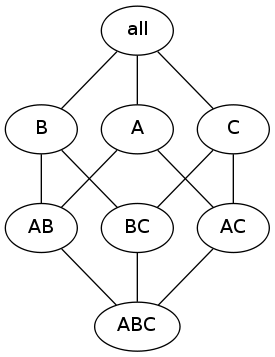
\includegraphics[scale=0.5]{dm0201.png} % scale指定缩放
% 				\caption{第一张浮动的图片}            % 图片的标题,会自动编号
% 				\label{dm0201}                % 图片的标记,一定要加在caption后面。不然指向的是前一个插图
% 			\end{figure}
% 
% 			试试使用浮动环境插入图片,但是这样图片就不知道浮动到什么地方去了:
% 
% 			\begin{figure}[htbp]                        % 
% 				\centering                              % 图片居中	
% 				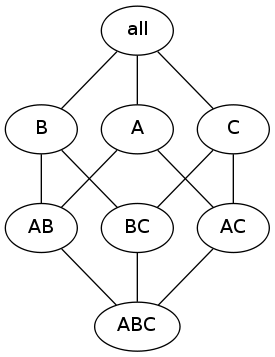
\includegraphics[scale=0.5]{dm0201.png} % scale指定缩放
% 				\caption{第二张浮动的图片}            % 图片的标题,会自动编号
% 				\label{dm0202}                % 图片的标记,一定要加在caption后面。不然指向的是前一个插图
% 			\end{figure}
% 
% 			试试使用浮动环境插入图片,但是这样图片就不知道浮动到什么地方去了:
% 
% 			\begin{figure}[htbp]                        % 
% 				\centering                              % 图片居中	
% 				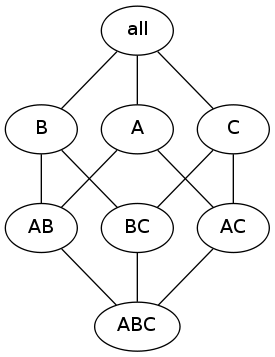
\includegraphics[scale=0.5]{dm0201.png} % scale指定缩放
% 				\caption{第三张浮动的图片}            % 图片的标题,会自动编号
% 				\label{dm0203}                % 图片的标记,一定要加在caption后面。不然指向的是前一个插图
% 			\end{figure}
% 
% 		\subsection{使用表格}
% 
% 			组表格也加上浮动环境:
% 
% 			\begin{table}[htbp]
% 				\caption{浮动环境中的三线表}
% 				\label{tab:threesome}
% 				\centering
% 				\begin{tabular}{lll}
% 					\hline
% 					操作系统 & 发行版 & 编辑器 \\
% 					\hline
% 					Windows & MikTeX & TeXnicCenter \\
% 					Unix/Linux & TeX Live & Emacs \\
% 					Mac OS & MacTeX & TeXShop \\
% 					\hline
% 				\end{tabular}
% 			\end{table}
% 

\end{document}
